\subsection{LQG-Regler}
    Die kombination eines LQR-Reglers und eines Luenberer-Observer nennt man \textit{LQG (Linear Quadratic Gaussian)}. Anstatt den realen Zustand $x(t)$ wird nun seine Schätzung $\widehat{x}(t)$ zurückgeführt.
    \begin{equation*}
        u(t) = -K\cdot\widehat{x}(t)
    \end{equation*}
    \begin{figure}[H]
        \centering
        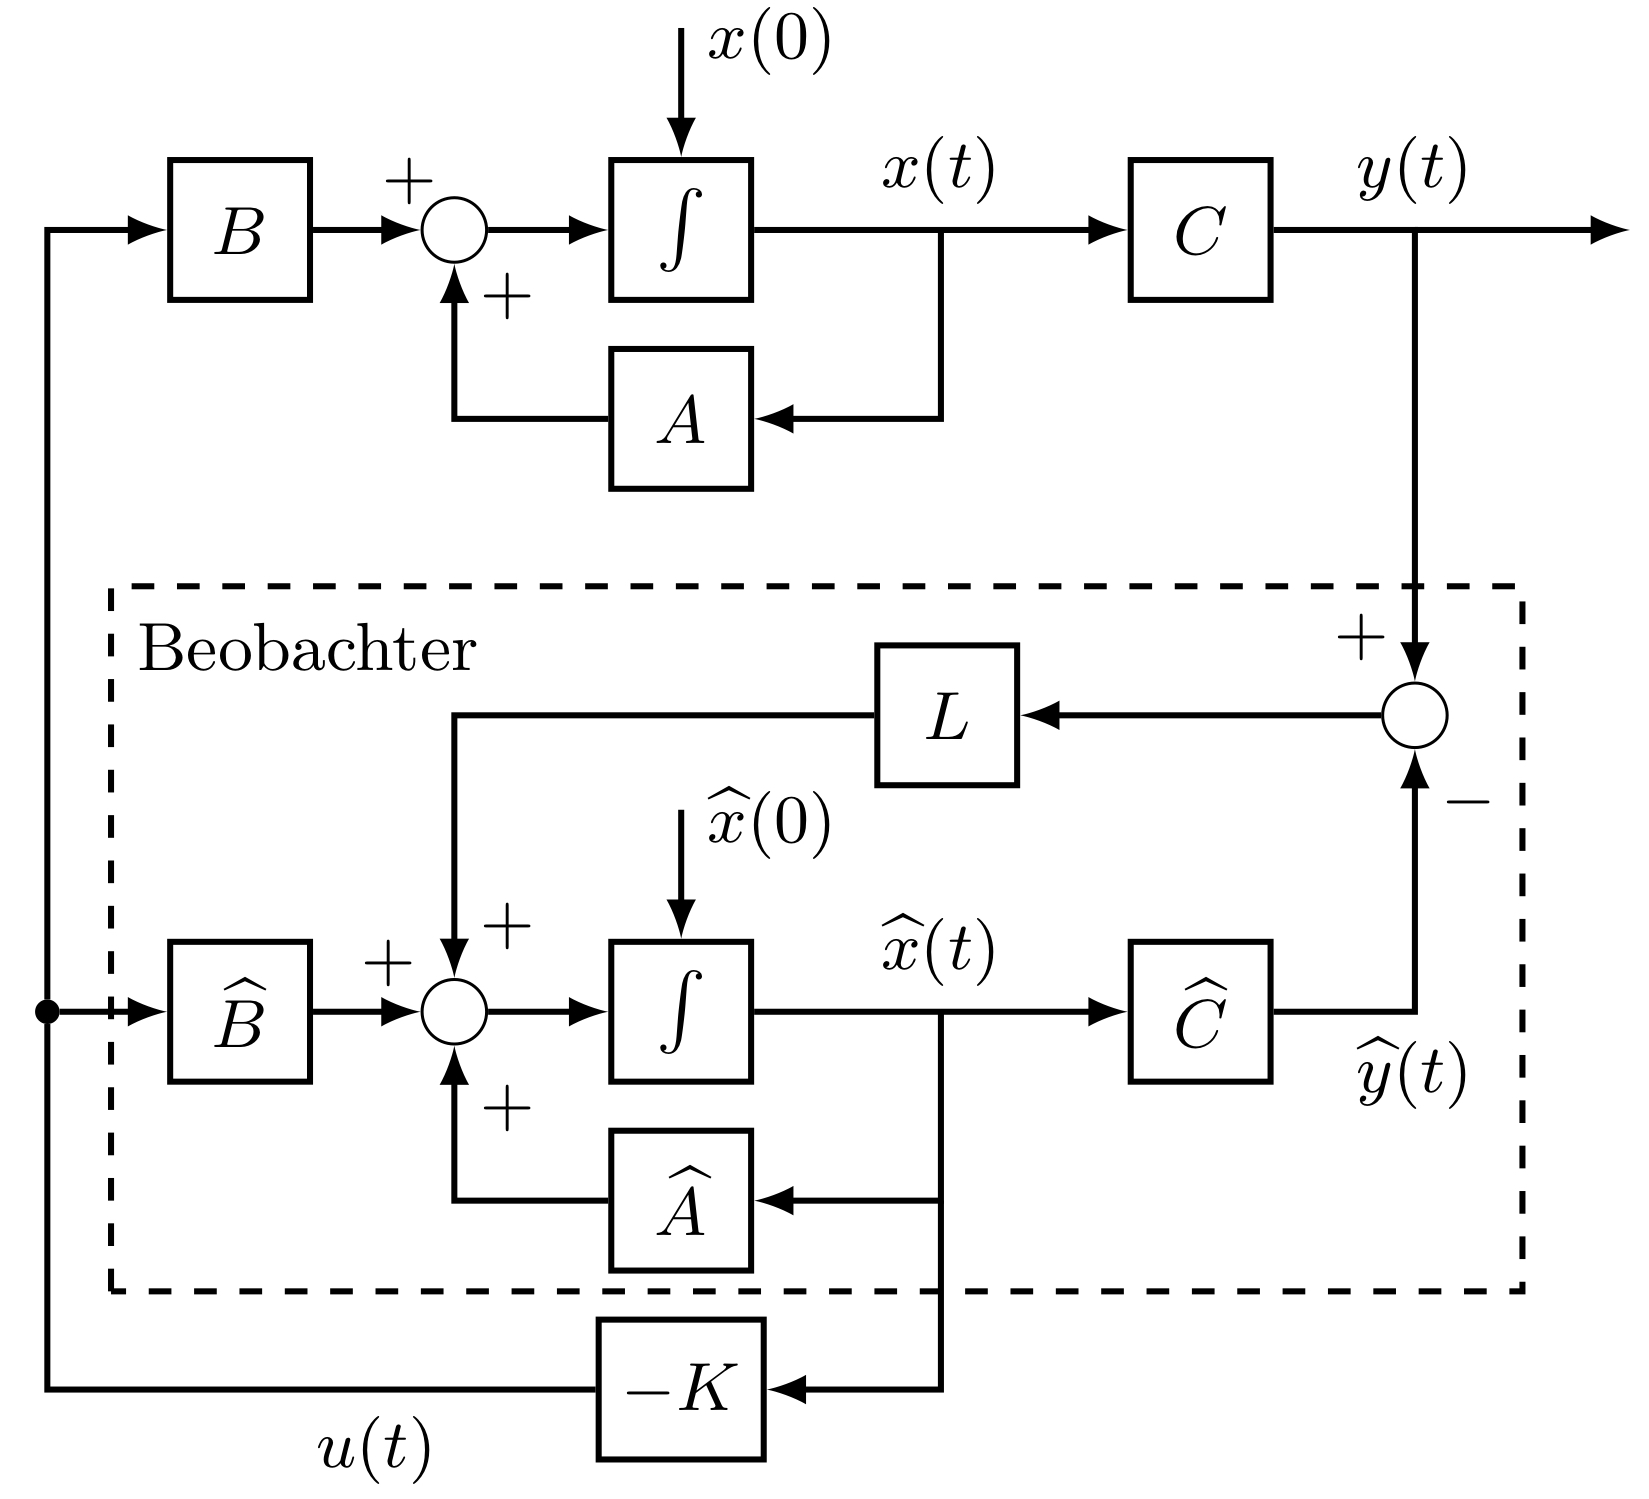
\includegraphics[width = 0.6\linewidth]{images/10/LQG_vanilla.jpeg}
        \caption{Blockdiagramm eines LQG-Reglers}
    \end{figure}
    
    \noindent\begin{minipage}{\linewidth}
    \begin{center}
        \tikzstyle{block} = [draw, fill=white!20, rectangle, minimum height=1em,  text centered, minimum width=1em]
\tikzstyle{sum} = [draw, fill=white!20, circle, node distance=0.75cm]
\tikzstyle{input} = [coordinate]
\tikzstyle{output} = [coordinate]
\tikzstyle{pinstyle} = [pin edge={to-,thin,black}]

% The block diagram code is probably more verbose than necessary
\begin{tikzpicture}[auto, node distance=0.75cm,>=latex']
    % We start by placing the blocks
    
    \node [input, name=input] {};
    \node [sum, right of=input, node distance= 0.5cm] (sum) {};
    \node [block, right of=sum] (L) {$\scriptscriptstyle -L$};
    \node[sum, right of=L,](sum1){};
    \node [block, right of=sum1, node distance = 0.9cm] (integr) {$\scriptstyle\int$};
    \node [block, right of=integr, node distance=1.5cm] (output1) {$\scriptscriptstyle -K$};
    \node [block, below of=integr, node distance = 0.6cm] (abklc) {$\scriptscriptstyle A-BK -LC$};
    \node[block, right of=output1, node distance = 1.0cm] (Bmatrix) {$\scriptscriptstyle B$};
    \node[sum, right of=Bmatrix] (sum2) {};
    \node [block, right of=sum2] (integr2) {$\scriptstyle\int$};
    \node [block, right of=integr2, node distance=1cm] (Cmatrix) {$\scriptscriptstyle C$};
    \node [output, right of=Cmatrix] (output) {};
    \node [block, below of=integr2, node distance = 0.6cm] (Amatrix) {$\scriptscriptstyle A$};

    % Once the nodes are placed, connecting them is easy. 
    \draw [draw,->] (input) -- node {$\scriptscriptstyle r$} (sum);
    \draw [->] (sum) -- node {$\scriptscriptstyle e$} (L);
    \draw [->] (L) -- node{} (sum1);
    \draw [->] (sum1) -- node{$\scriptscriptstyle \dot{\hat{x}}$} (integr);
    \draw [->] (integr) -- node [name=x_hat, pos=0.75] {$\scriptscriptstyle \hat{x}$}(output1);
    \draw [->] (x_hat) |- (abklc);
    \draw [->] (abklc) -| node[pos=0.95] {$\scriptscriptstyle +$} node [near end] {} (sum1);
    \draw [->] (output1) -- node{$\scriptscriptstyle u$} (Bmatrix);
    \draw [->] (Bmatrix) -- node{} (sum2);
    \draw [->] (sum2) -- node{$\scriptscriptstyle \dot{x}$} (integr2);
    \draw [->] (integr2) -- node [name=x] {$\scriptscriptstyle x$}(Cmatrix);
    \draw [->] (x) |- (Amatrix);
    \draw [->] (Amatrix) -| node[pos=0.95] {$\scriptscriptstyle +$} node [near end] {} (sum2);
    \draw [->] (Cmatrix) -- node [name=y] {$\scriptscriptstyle y$}(output);
    \draw [->] (y) |- ++(0,-1.2) -| node[pos=0.95] {$\scriptscriptstyle -$} node [near end] {} (sum);
\end{tikzpicture}
        \captionof{figure}{Alternative Dastellung des LQG-Reglers aufgeteilt in Controller und Plant.}
    \end{center}
    \end{minipage}
    
    % \begin{figure}[H]
    %     \centering
    %     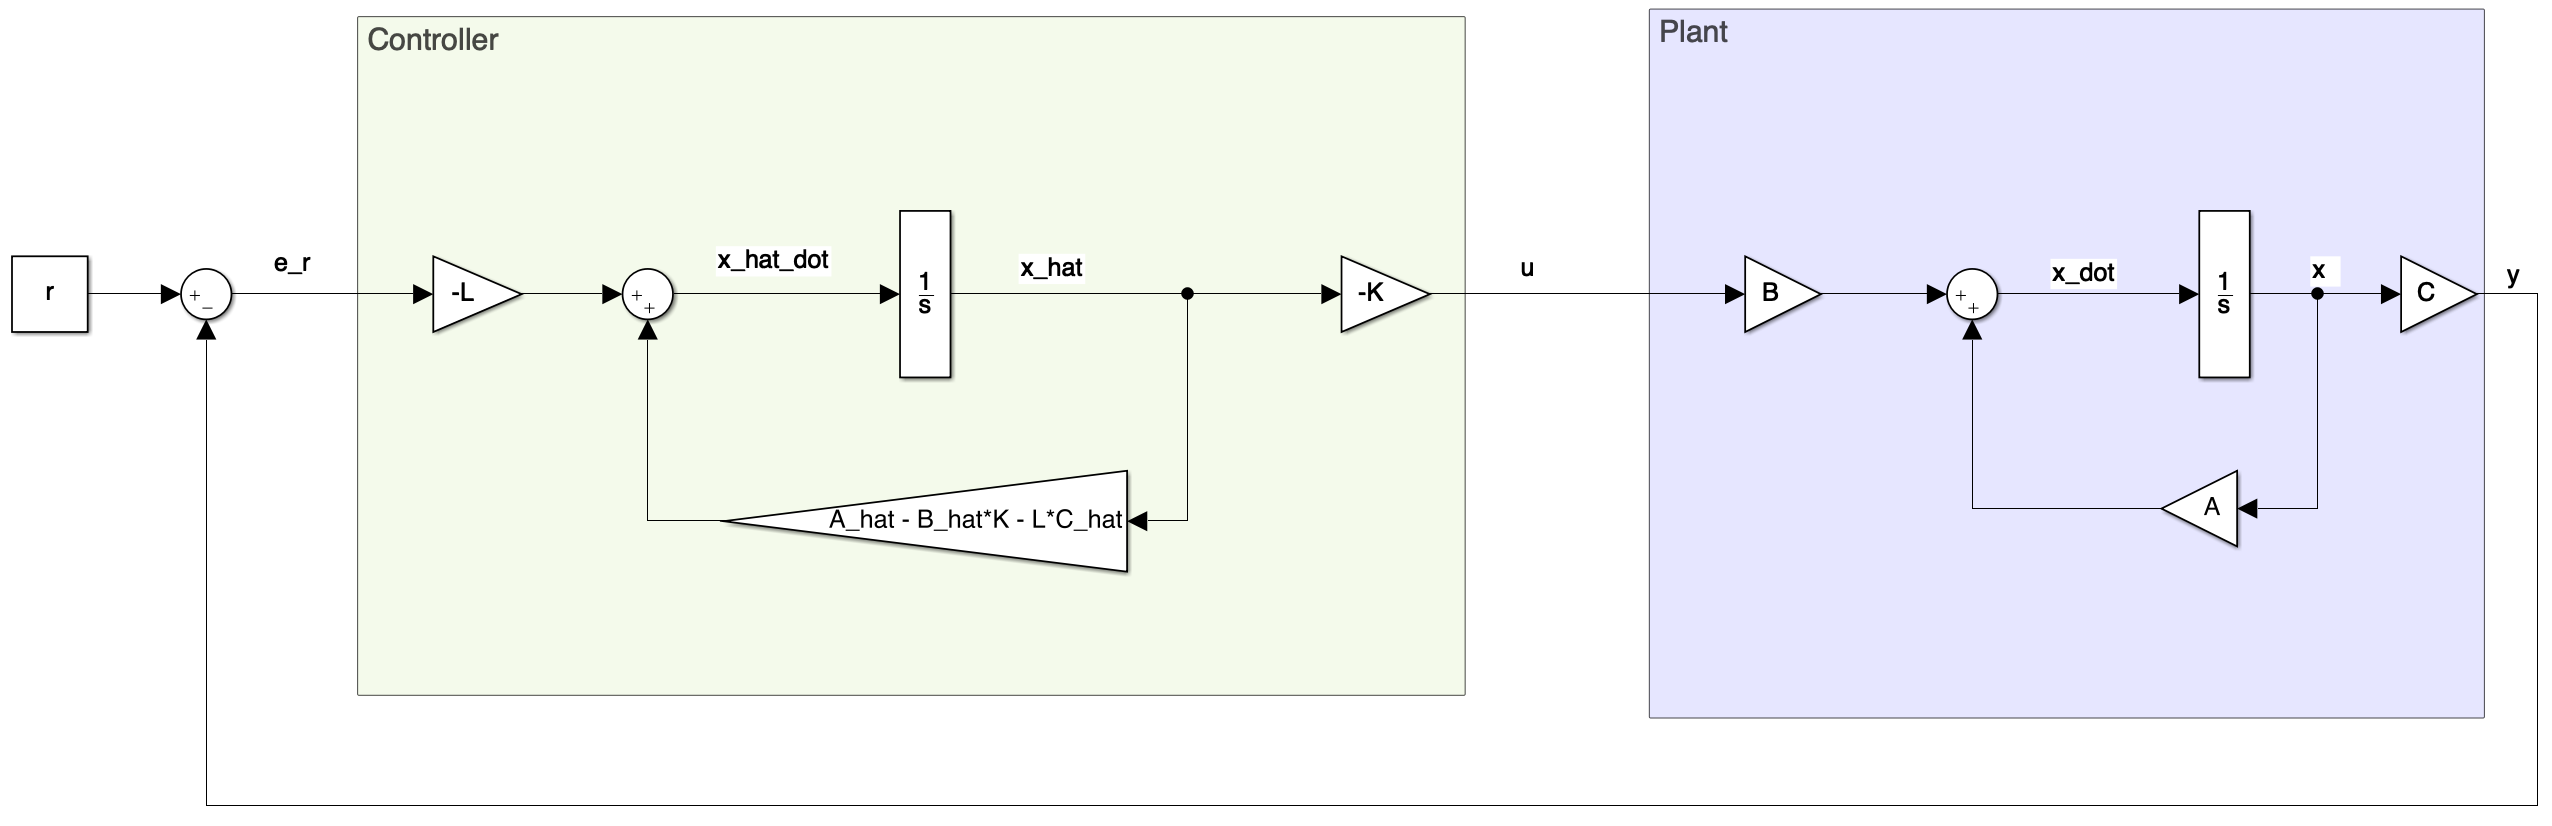
\includegraphics[width = \linewidth]{images/10/LQR_alt.png}
    %     \caption{Alternative Darstellung des LQR-Reglers}
    % \end{figure}
    
\subsection{Stabilität des LQG}
    Unter der Annahme, dass die Matrizen $\{A, B, C\}$ exakt bekannt sind ergibt sich folgende Dynamik
    \begin{equation*}
        \Tilde{x}(t) = \begin{bmatrix}x(t)\\\widehat{x}(t)\end{bmatrix},\quad
        \frac{d}{dt}\Tilde{x}(t) = 
        \underbrace{\begin{bmatrix}
        A   &   -B\cdot K\\
        L\cdot C & A-B\cdot K-L\cdot C
        \end{bmatrix}}_{\Tilde{A}_{\textnormal{cl}}}
        \cdot \Tilde{x}(t)
    \end{equation*}
    Die Stabilität ist durch die Eigenwerte von $\Tilde{A}_{\textnormal{cl}}$ gegeben. Sind aber in dieser Form nicht einfach zu berechnen.
    
    \subsubsection{Separation Principle}
        Verwendet man die Koordinatentransformation
        \begin{equation*}
            \Tilde{z} = 
            \begin{bmatrix}
            x(t)\\e(t)
            \end{bmatrix}
            =
            \begin{bmatrix}
            x(t)\\x(t)-\widehat{x}(t)
            \end{bmatrix}
            =
            \begin{bmatrix}
            I_{n\times n} & 0\\I_{n\times n} & I_{n\times n}
            \end{bmatrix}
            = \underbrace{T^{-1}}_{=T}\cdot\widehat{x}(t)
        \end{equation*}
        Daraus ergib sich folgende Dynamik
        \begin{equation*} 
            \frac{d}{dt}\Tilde{z}(t) = 
            \underbrace{\begin{bmatrix}
            A-B\cdot K   &   B\cdot K\\
            0 & A-L\cdot C
            \end{bmatrix}}_{\textnormal{gleiche EW wie }\Tilde{A}_{\textnormal{cl}}}
            \cdot\Tilde{z}(t) = T^{-1}\cdot\Tilde{A}_\textnormal{cl}\cdot T\cdot\Tilde{z}(t)
        \end{equation*}
        Daraus folgt direkt
        \begin{align*}
            \operatorname{eig}(T^{-1}\cdot\Tilde{A}_\textnormal{cl}\cdot T) &= \operatorname{eig}(\Tilde{A}_\textnormal{cl}) = \operatorname{eig}(A-B\cdot K)\cup \operatorname{eig}(A-L\cdot C)\\ 
            &\therefore \Tilde{A}_\textnormal{cl}\,\textnormal{ist Hurwitz}
        \end{align*}